%%==================================================
%% chapter02.tex for BIT Master Thesis
%% modified by yang yating
%% version: 0.1
%% last update: Dec 25th, 2016

%% modified by Meng Chao
%% version: 0.2
%% last update: May 29th, 2017
%%==================================================
\chapter{多旋翼无人机控制系统设计}
\label{chap:control design}

%2.1
\section{多旋翼无人机建模}
多旋翼无人机结构如图\ref{fig2.1}所示,分为四个部分:刚体运动学模型,刚体动力学模型,控制效率模型和动力单元模型\upcite{[2.1]}。刚体运动学模型与无人机的质量和受力无关,以质点为模型研究无人机位置、速度、姿态、角速度等状态的变化;刚体动力学模型,研究无人机所受力和力矩与运动状态变化的关系,多旋翼无人机与一般刚体动力学模型最大的不同在于螺旋桨拉力方向始终与机体坐标系$z_b$轴的负方向一致,以上两个模型又统称为无人机刚体模型。控制效率模型表示不同机型对螺旋桨拉力和力矩的分配情况;动力单元模型则研究多旋翼无人机动力装置电机的数学模型。
\begin{figure}[h]
\centering
%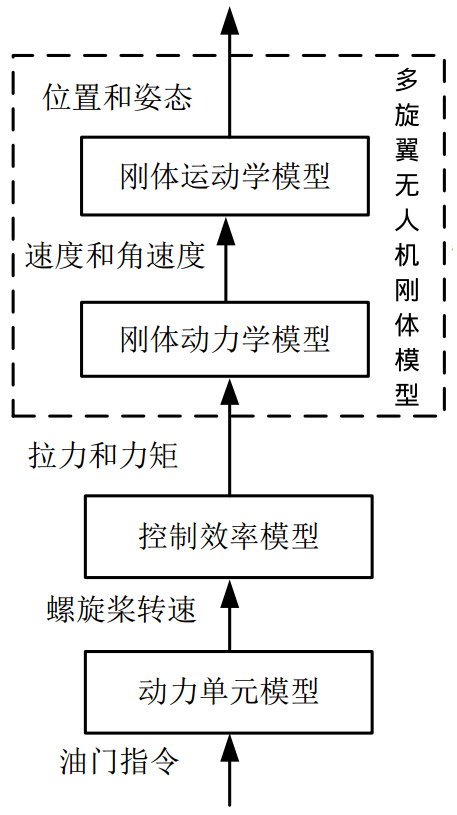
\includegraphics[scale=0.4]{figures/Fig2.1.png}
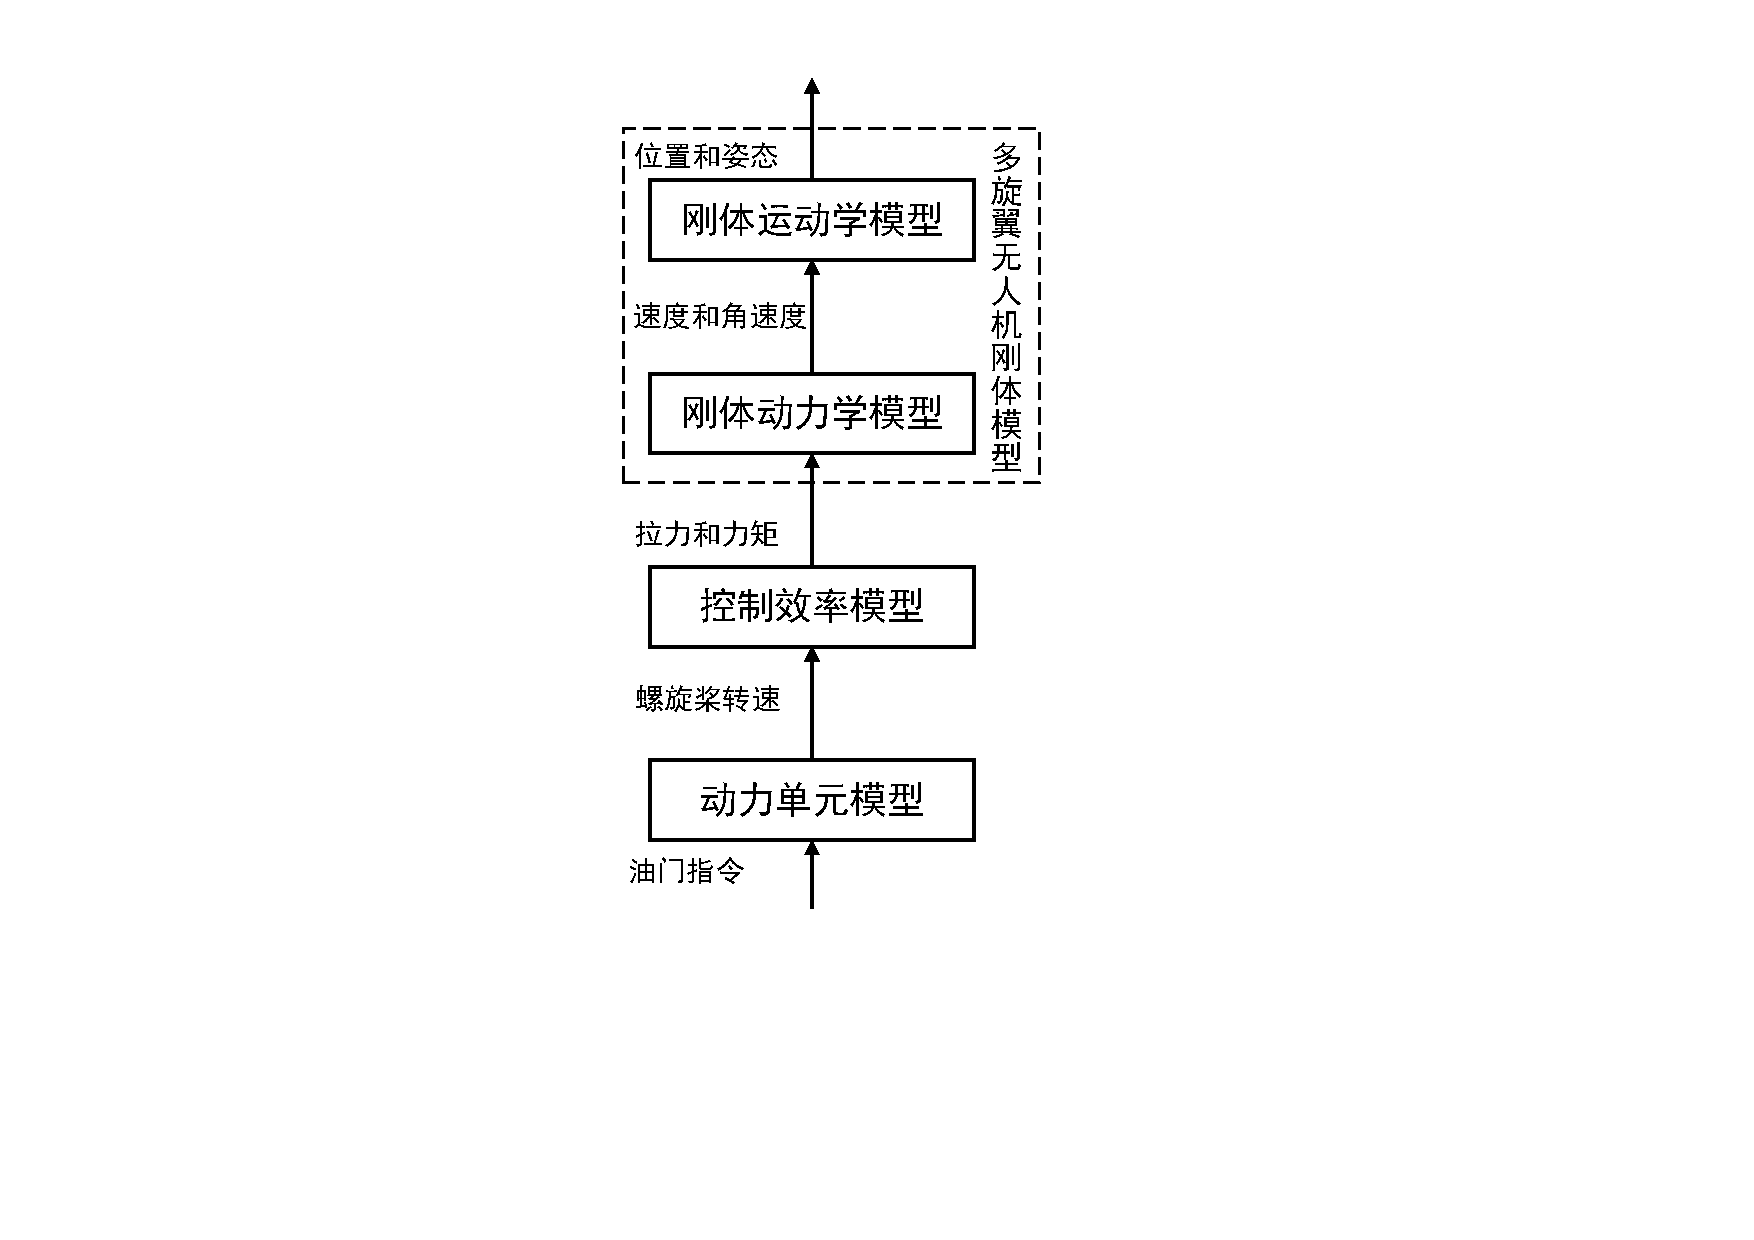
\includegraphics[scale=0.8,,angle=-90]{figures/Fig2-1.pdf}
\caption{多旋翼无人机模型}
\label{fig2.1}
\end{figure}

\subsection{坐标系定义与坐标变换}
多旋翼无人机的空间运动主要分为:质心运动和绕质心的转动,因而在描述任意时刻的空间运动时需要6个自由度:3轴质心运动和3轴角运动。在进行多旋翼无人机建模之前首先应该选择合适的坐标系,可以方便、准确的表示多旋翼无人机的空间状态和受力情况\upcite{[2.2]}。本文在进行多旋翼无人机建模时使用两个坐标系:固联于无人机的机体坐标系和固定于无人机起飞点的地面坐标系,如图\ref{fig2.2}所示。\\
(1)机体坐标系$\boldsymbol{O} \boldsymbol{x}_b \boldsymbol{y}_b \boldsymbol{z}_b$

机体坐标系原点定义在多旋翼无人机质心上,$\boldsymbol{O} \boldsymbol{x}_b$平行于无人机前后旋翼,指向无人机前进的方向;$\boldsymbol{O} \boldsymbol{z}_b$位于无人机纵向平面,垂直向下;$\boldsymbol{O} \boldsymbol{y}_b$垂直于无人机纵向平面,方向根据右手定则确定。 \\ 
(2)地面坐标系$\boldsymbol{O} \boldsymbol{x}_e \boldsymbol{y}_e \boldsymbol{z}_e$

地面坐标系原点固定于无人机起飞位置,$\boldsymbol{O} \boldsymbol{x}_e$位于地平面内并指向无人机前进方向;$\boldsymbol{O} \boldsymbol{z}_e$垂直与地面并指向地心;$\boldsymbol{O} \boldsymbol{y}_e$位于地面平内,方向根据右手定则确定。

\begin{figure}[h]
\centering
%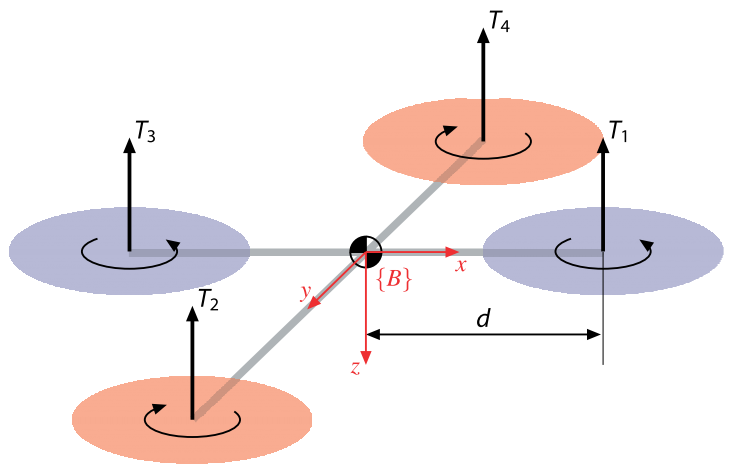
\includegraphics[scale=0.5]{figures/Fig2.2.png}
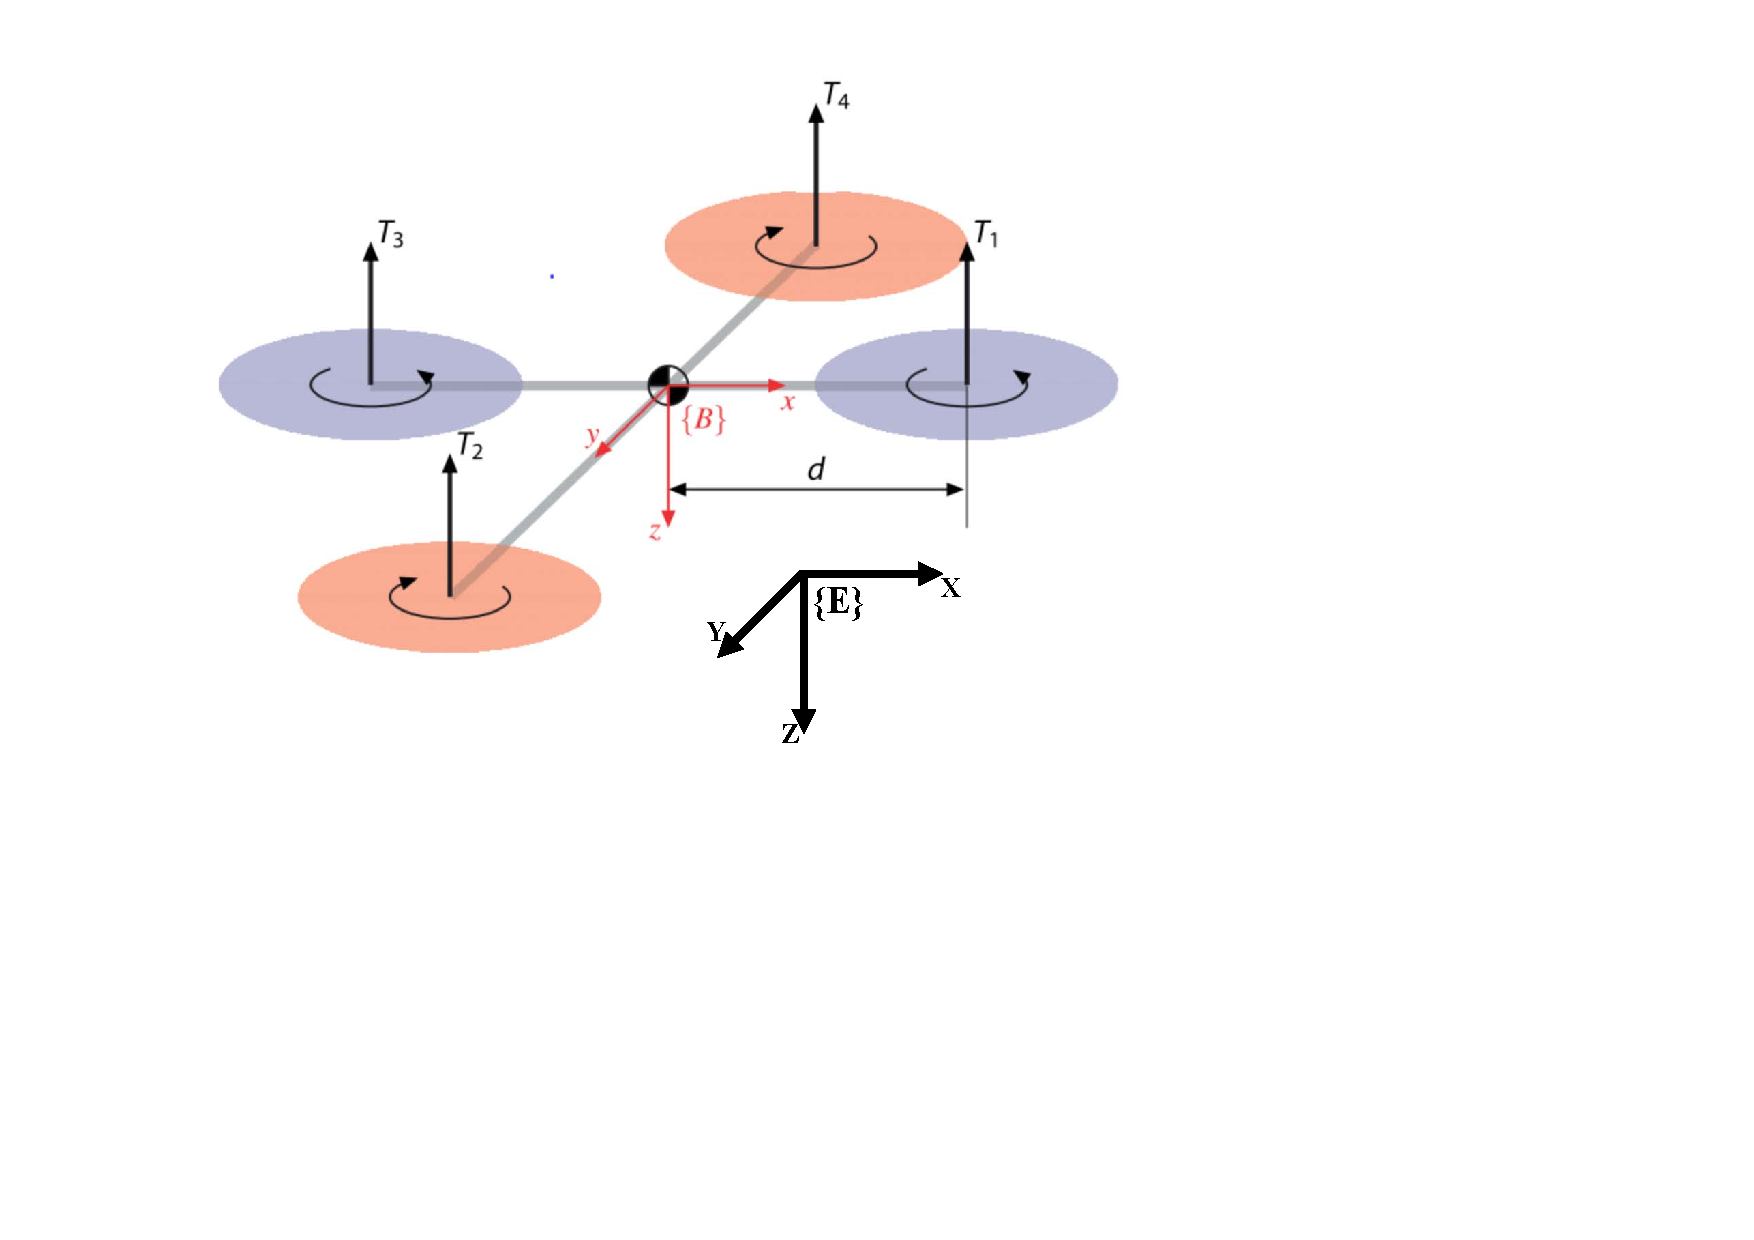
\includegraphics[scale=0.7,angle=-90]{figures/Fig2-2.pdf}
\caption{多旋翼无人机坐标系定义}
\label{fig2.2}
\end{figure}

为了便于描述无人机的空间运动状态,必须选择合适的坐标系,例如选择使用机体坐标系描述空间绕质心的转动,使用地面坐标系描述空间质心运动。不同坐标系之间需要进行坐标转换,如将机体坐标系受到的螺旋桨拉力转换到地面坐标系分析质心运动。因而,坐标转换是无人机建模不可或缺的一部分。一般机体坐标系与地面坐标系之间的转换关系可以由三个姿态角确定,偏航角$\psi$,俯仰角$\theta$和滚转角$\phi$。\\
1).俯仰角$\theta$:机体坐标系$\boldsymbol{O} \boldsymbol{x}_b$轴与地平面之间的夹角,沿$\boldsymbol{O} \boldsymbol{y}_b$轴顺时针转动抬头为正。\\
2).滚转角$\phi$:机体坐标系$\boldsymbol{O} \boldsymbol{z}_b$与通过机体坐标系$\boldsymbol{O} \boldsymbol{x}_b$轴的铅垂面之间的夹角,沿$\boldsymbol{O} \boldsymbol{x}_b$轴顺时针转动向右滚转为正。\\
3).偏航角$\psi$:机体坐标系$\boldsymbol{O} \boldsymbol{x}_b$轴在地平面的投影与地面坐标系$\boldsymbol{O} \boldsymbol{x}_e$的夹角,沿$\boldsymbol{O} \boldsymbol{z}_b$轴顺时针转动右偏为正。

地面坐标系到机体坐标系的转换可以通过欧拉转动定理绕轴连续转动得到,首先绕地面坐标系$\boldsymbol{O} \boldsymbol{z}_e$转动偏航角$\psi$,得到过渡坐标系$\boldsymbol{O} \boldsymbol{x}^{'} \boldsymbol{y}^{'} \boldsymbol{z}^{'}$;之后再由过渡坐标系绕$\boldsymbol{O} \boldsymbol{y}^{'}$旋转俯仰角$\theta$,得到过渡坐标系$\boldsymbol{O} \boldsymbol{x}^{''} \boldsymbol{y}^{''} \boldsymbol{z}^{''}$;最后由过度坐标系$\boldsymbol{O} \boldsymbol{x}^{''} \boldsymbol{y}^{''} \boldsymbol{z}^{''}$绕$\boldsymbol{O} \boldsymbol{x}^{''}$旋转滚转角$\phi$,得到机体坐标系$\boldsymbol{O} \boldsymbol{x}_b \boldsymbol{y}_b \boldsymbol{z}_b$。从地面坐标系到机体坐标系的旋转矩阵$\boldsymbol{R}_{BE}$为
\begin{equation}
\label{equ2.1}
\begin{aligned}
\boldsymbol{R}_{BE} 
&= \boldsymbol{R}(\boldsymbol{\phi}) \boldsymbol{R}(\boldsymbol{\theta}) \boldsymbol{R}(\boldsymbol{\psi}) \\ 
&= 
\begin{bmatrix}
\cos\theta \cos\psi & \cos\theta \sin\psi & -\sin\theta \cr
\sin\theta \cos\psi \sin\phi - \sin\psi \cos\phi & \sin\theta \sin\psi \sin\phi + \cos\psi \cos\phi & \cos\theta \sin\phi \cr
\sin\theta \cos\psi \cos\phi + \sin\psi \sin\phi & \sin\theta \sin\psi \cos\phi - \cos\psi \sin\phi & \cos\theta \cos\phi \cr
\end{bmatrix}
\end{aligned}
\end{equation}

\subsection{多旋翼无人机刚体模型}
进行多旋翼无人机刚体建模时,做出如下假设\upcite{[2.3]}:
\begin{enumerate}  [itemindent=1em,label={(\arabic*)}]
\item 假设多旋翼无人机是刚体。
\item 假设多旋翼无人机的质量和转动惯量保持不变。
\item 假设多旋翼无人机的几何中心和重心重合。
\item 假设多旋翼无人机只受重力和螺旋桨的拉力。
\item 假设奇数编号的螺旋桨逆时针转动,偶数编号螺旋桨顺时针转动
\end{enumerate}
首先进行刚体运动学建模,刚体运动学模型描述了多旋翼无人机运动状态的变化。\\
(1) 质心平动模型

研究地面坐标系下无人机的位置$\boldsymbol{P}_e = [X,Y,Z]^T$的变化,分解到三轴坐标上有。
\begin{equation}
\label{equ2.2}
\begin{aligned}
\dot{\boldsymbol{P}}_e &= \boldsymbol{V}_e \\
\begin{bmatrix}
\dot{X} \cr \dot{Y} \cr \dot{Z} \cr
\end{bmatrix}
&=
\begin{bmatrix}
V_X \cr V_Y \cr V_Z \cr
\end{bmatrix}
\end{aligned}
\end{equation}
(2) 绕质心转动模型

研究姿态角速率$\dot{\boldsymbol{\Theta}}=[\dot{\theta},\dot{\psi},\dot{\phi}]^T$与机体坐标系下的转动角速率$\boldsymbol{\omega}_b=[\omega_x , \omega_y , \omega_z]^T$的关系。根据地面坐标系与机体坐标系之间的变换关系有。
\begin{equation}
\label{equ2.3}
\begin{aligned}
\boldsymbol{\omega}_b & = \boldsymbol{R}_{EB} \dot{\boldsymbol{\psi}}+\boldsymbol{R}(\boldsymbol{\phi}) \dot{\boldsymbol{\theta}}+ \dot{\boldsymbol{\phi}} 
\\
\begin{bmatrix}
\omega_x \cr \omega_y \cr \omega_z \cr
\end{bmatrix}
& =
\begin{bmatrix}
0 & -\sin \theta & 1 \cr
\cos \phi & \cos \theta \sin \phi & 0 \cr
-\sin \phi & \cos \theta \cos \phi & 0 \cr
\end{bmatrix}
\begin{bmatrix}
\dot{\theta} \cr \dot{\psi}  \cr  \dot{\phi} \cr
\end{bmatrix}
\end{aligned}
\end{equation}
(3)质心平动动力学模型

质心平动动力学模型研究无人机受力与质心平动的关系。设机体坐标系下所有螺旋桨产生的总拉力$\boldsymbol{T}_b=[0,0,T]^{T}$,无人机受到的重力在世界坐标系下表示为$\boldsymbol{G}_e=[0,0,mg]^T$,则无人机的质心运动方程可以表示为
\begin{equation}
\label{equ2.4}
\begin{aligned}
m\boldsymbol{\dot{V}}_e &= \boldsymbol{G}_e -  \boldsymbol{R}_{EB} \boldsymbol{T}_b
\end{aligned}
\end{equation}
(4)绕质心转动动力学模型

绕质心转动的动力学模型研究无人机所受力矩与其空间角运动的关系。设无人机在机体坐标系下的转动惯量为
\begin{equation}
\label{equ2.5}
\boldsymbol{I}_b = 
\begin{bmatrix}
I_x & 0 & 0 \cr
0 & I_y & 0 \cr
0 & 0 & I_z \cr
\end{bmatrix}
\end{equation}
假设无人机受到的总力矩在地面坐标系下为$\boldsymbol{M}_e=[M_x,M_y,M_z]^T$,根据矢量绝对导数与相对导数关系,由角动量定理得
\begin{equation}
\label{equ2.6}
\begin{aligned}
\boldsymbol{M}_e &= {d\boldsymbol{H}_e \over dt} = {d\boldsymbol{H}_b \over dt} +  \boldsymbol{\omega}_b \times \boldsymbol{H}_b 
\\
\boldsymbol{M}_e &= \boldsymbol{I}_b \dot{\boldsymbol{\omega}}_b +\boldsymbol{\omega}_b \times \boldsymbol{I}_b \boldsymbol{\omega}_b 
\end{aligned}
\end{equation}
以上公式\eqref{equ2.2},\eqref{equ2.3},\eqref{equ2.4},\eqref{equ2.6}组成了多旋翼无人机的非线性刚体模型。

\subsection{多旋翼无人机控制效率模型}
多旋翼无人机控制效率模型研究无人机机型结构与螺旋桨拉力和力矩分配的关系\upcite{[2.4]}。以十字型四旋翼无人机为例,设第$i$个螺旋桨的拉力$\boldsymbol{F}_i$与电机转速$\omega_i$关系为$\boldsymbol{F}_i = c_T \omega_i^2$,则无人机受到的总拉力为
\begin{equation}
\label{equ2.7}
\boldsymbol{T}_b = \sum\limits_{i=1}^4 \boldsymbol{F}_i =  \sum\limits_{i=1}^4 c_T \omega_i^2
\end{equation}
四旋翼无人机臂长$d$,螺旋桨对机体坐标系三轴产生的力矩为
\begin{equation}
\label{equ2.8}
\begin{aligned}
M_x &= d c_T \left( \omega_4^2 - \omega_2^2\right)
\\
M_y &= d c_T \left( \omega_1^2 - \omega_3^2\right)
\\
M_z &= d c_M \left( \omega_1^2 - \omega_2^2 + \omega_3^2 - \omega_4^2\right)
\end{aligned}
\end{equation}
公式\eqref{equ2.7},\eqref{equ2.8}中$c_T $表示与螺旋桨翼型相关的常量参数,$c_M$表示螺旋桨反扭力常数。将以上两公式进行整理可以得到无人机动力分配模型
\begin{equation}
\label{equ2.9}
\begin{bmatrix}
T \cr M_x \cr M_y \cr M_z \cr 
\end{bmatrix}
=
\begin{bmatrix}
c_T & c_T & c_T & c_T  \cr
0 & -d c_T & 0 & d c_T \cr
d c_T & 0 & -d c_T & 0 \cr
c_M & c_M & c_M & c_M  \cr
\end{bmatrix}
\begin{bmatrix}
\omega_1^2 \cr \omega_2^2 \cr \omega_3^2 \cr \omega_4^2 \cr
\end{bmatrix}
\end{equation}


\subsection{多旋翼无人机动力单元模型}
多旋翼无人机一般选用直流无刷电机,无刷电机微分方程为
\begin{equation}
\label{equ2.10}
\begin{aligned}
u &= iR + L {di \over dt} + k_e \omega
\\
J_m {d\omega \over dt} &= M_m - M_{load}
\end{aligned}
\end{equation}
其中$u$表示电机电压,$i$为电机电流,$\omega$表示电机旋转角速度,$R$表示电机等效电阻,$L$表示电机线圈电感,$k_e$表示电机反电动势系数,$J_m$表示电机线圈的轴向转动惯量,$M_m=k_m i$表示电机输出力矩,$M_{load}$表示电机负载力矩。由于电机线圈电感较小,忽略电机线圈电感后得到的多旋翼无人机动力单元模型为
\begin{equation}
\label{equ2.11}
\begin{aligned}
i &= {(u-k_e \omega) \over R }
\\
J_m {d \omega \over dt} &= k_m{u \over R } - {k_e k_m \omega \over R} - M_{load}
\end{aligned}
\end{equation}

%2.2
\section{多旋翼无人机控制算法研究}
为了更好的控制无人机运动,选择串级PID作为控制率,分为两个控制器:位置控制器和姿态控制器\upcite{[2.5]}。位置控制器为外环,负责控制无人机的位置,输出期望的姿态角;姿态控制器为内环,负责控制无人机的姿态角,输出电机控制信号。通过内外环控制器实现多旋翼飞行器的升降、悬停和侧飞等飞行模态,控制系统结构如图\ref{fig2.3}所示。
\begin{figure}[h]
\centering
%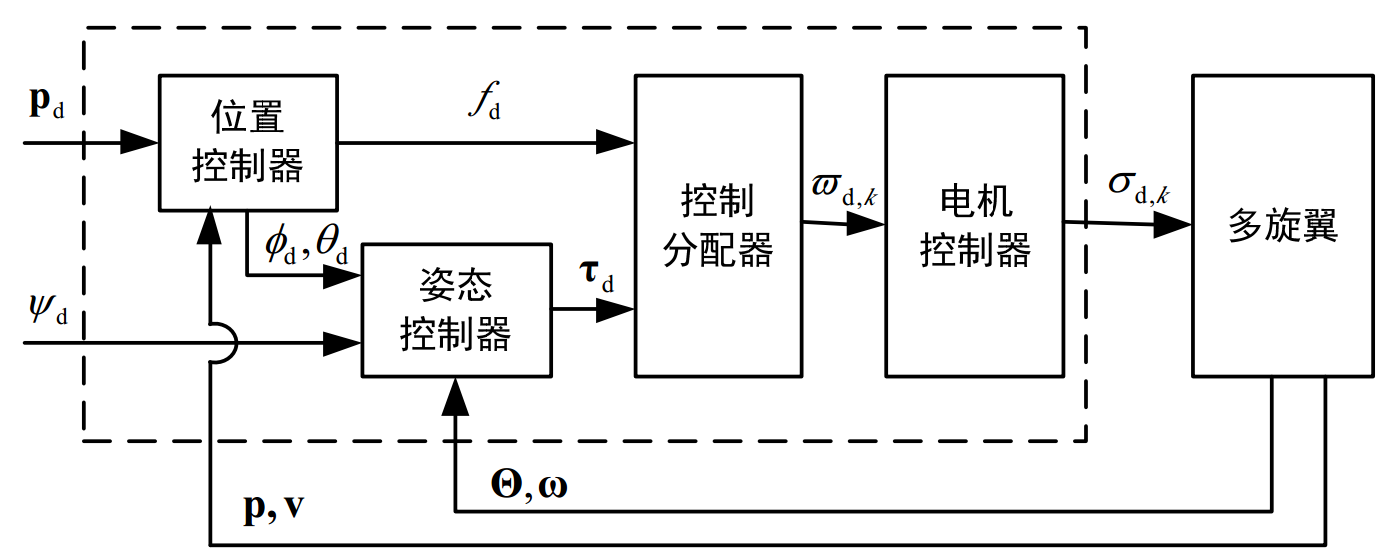
\includegraphics[scale=0.3]{figures/Fig2.3.png}
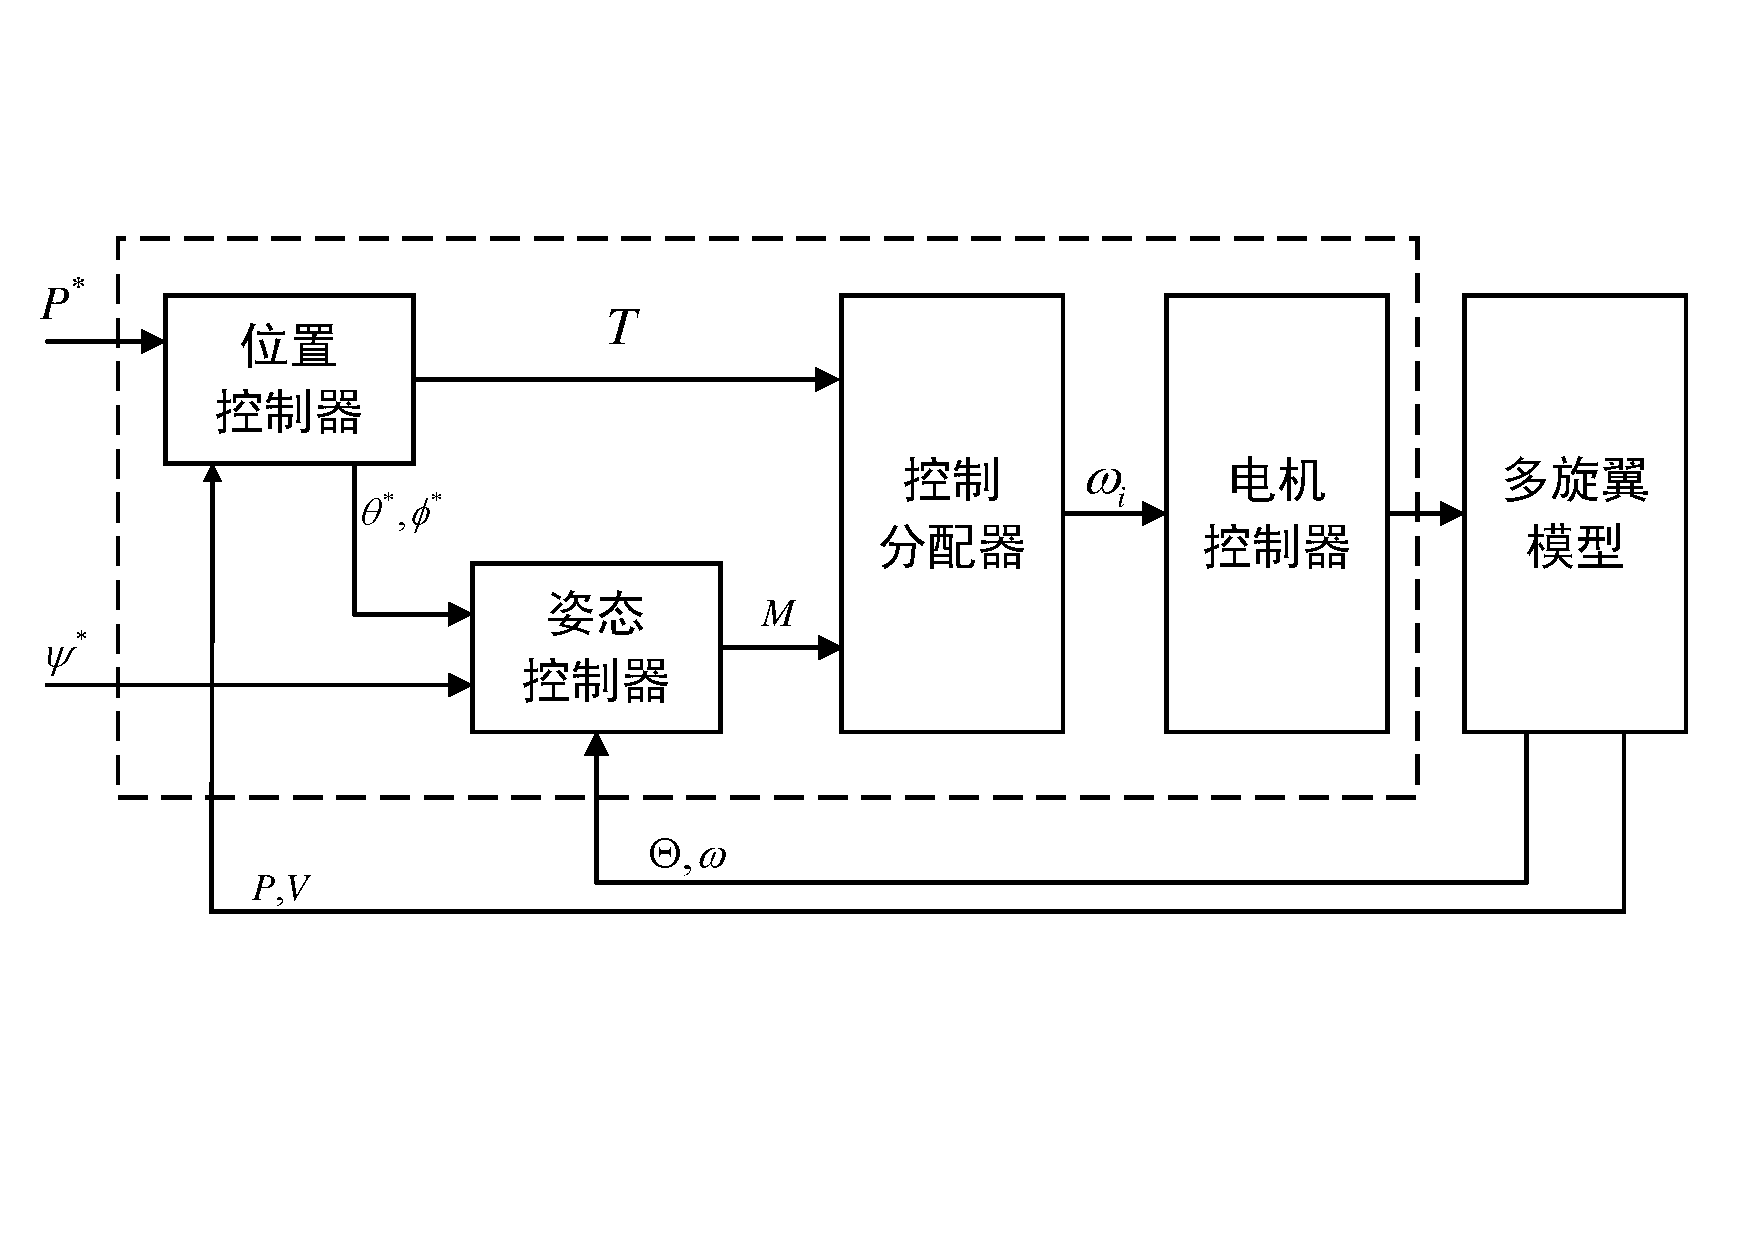
\includegraphics[scale=0.5,angle=-90]{figures/Fig2-3.pdf}
\caption{多旋翼无人机闭环控制系统}
\label{fig2.3}
\end{figure}

\subsection{姿态控制器}
多旋翼无人机的姿态角直接影响无人机的飞行状态,根据方程\eqref{equ2.5}可知无人机绕质心转动的动力学模型为二阶系统,因而在姿态控制回路引入比例-微分控制器进行调节,并将控制通道解耦为俯仰/滚转通道和偏航通道。对于俯仰/滚转通道,多旋翼无人机的俯仰、滚转运动对称,因而以俯仰通道为例介绍,设计比例-微分控制器
\begin{equation}
\label{equ2.12}
\begin{aligned}
M_x &= K_{p\theta} \left( \theta^* - \theta \right) + K_{d\theta} \left( \dot{\theta}^* -  \dot{\theta} \right)
\end{aligned}
\end{equation}
其中$\theta$、$\dot{\theta}$表示反馈的姿态角和姿态角速率,$\theta^*$表示期望俯仰角,由位置控制器给出。$ \dot{\theta}^*$通常较小可以忽略。

对于偏航通道,同样采用比例-微分控制器
\begin{equation}
\label{equ2.13}
M_z = K_{p\psi} \left( \psi^* - \psi \right) + K_{d\psi} \left( \dot{\psi}^* -  \dot{\psi} \right)
\end{equation}
其中$\psi$、$\dot{\psi}$表示反馈的姿态角和姿态角速率。不同于俯仰/滚转通道,期望偏航角$\psi^*$不由位置控制器提供,而是根据预设轨迹或外部遥控装置直接给出。$ \dot{\psi}^*$通常较小可以忽略。

\subsection{位置控制器}
对多旋翼无人机刚体运动学模型\eqref{equ2.3},\eqref{equ2.4}进行线性化近似,其水平运动影响俯仰/滚转姿态角变化,高度运动影响无人机推力变化。对于水平运动,$x$,$y$方向的运动是对称的,以$x$方向运动为例,设计比例控制器约束无人机的期望速度
\begin{equation}
\label{equ2.14}
v_x^* =  K_{px} \left( p_x^* - p_x \right)
\end{equation}
其中$p_x $表示反馈的$x$轴位置,$p_x^*$表示$x$轴上的期望位置,$v_x^*$表示$x$轴的期望速度。为了使机体沿$x$轴运动,需要改变俯仰角,有
\begin{equation}
\label{equ2.15}
f_x = T \sin\theta \approx T \theta
\end{equation}
根据方程\eqref{equ2.15}设计比例控制器
\begin{equation}
f_x = K_{vx} \left(  v_x^* - v_x \right)
\end{equation}
联立方程\eqref{equ2.14},\eqref{equ2.15},\eqref{equ2.16}可以得到期望的俯仰姿态角$\theta^*$
\begin{equation}
\label{equ2.16}
\theta^* = K_{vx} \left( K_{px} \left( p_x^* - p_x \right) - v_x \right)
\end{equation}

对于高度控制器,设计比例-微分控制器调节多旋翼无人机的推力
\begin{equation}
\label{equ2.17}
T = K_{pz} \left( z^* -z  \right) + K_{dz} \left( \dot{z}^* - \dot{z}  \right) + G_0
\end{equation}
其中,$z^*$表示目标高度,$z$,$\dot{z}$表示无人机反馈的高度位置和速度。$G_0$是前馈控制量,抵消重力的影响,避免高度控制中的定常干扰。

%2.3
\section{仿真验证}
根据上文的多旋翼无人机数学模型,利用MATLAB的S函数在Simulink\upcite{[2.6]}环境下搭建无人机仿真模型;根据上节设计的控制率,搭建串级PID无人机控制器,整个仿真系统如图\ref{fig2.4}所示。
\begin{figure}[h]
\centering
	%\subfigure[LSD-SLAM]
    
		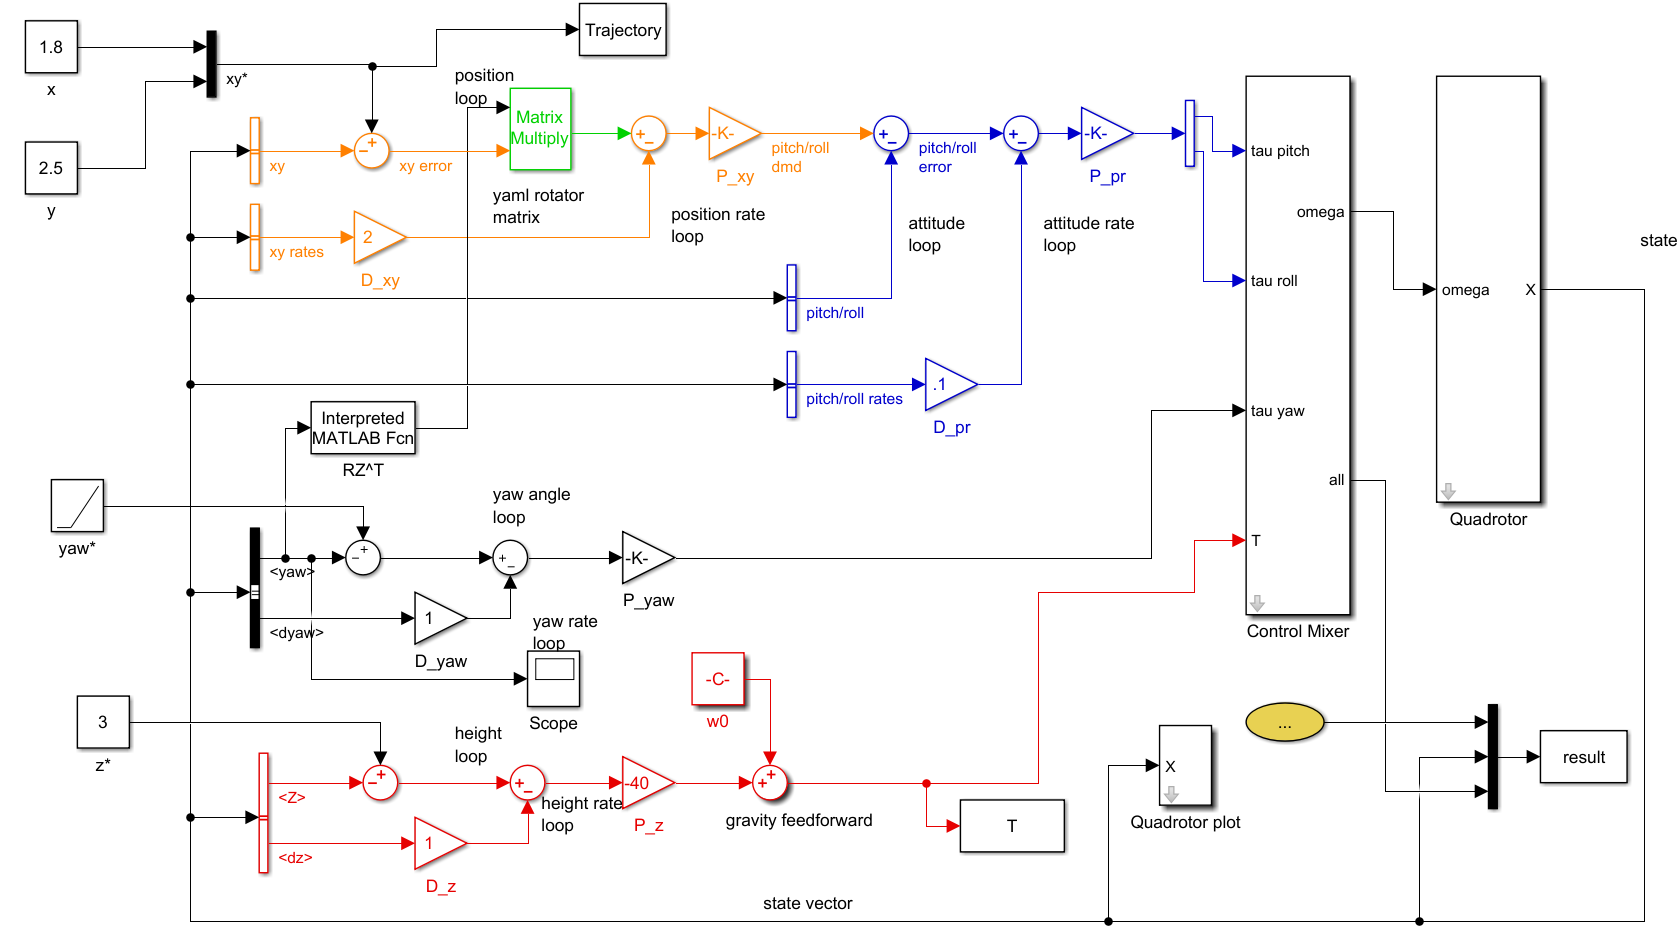
\includegraphics[scale=0.4]{figures/Fig2.4.png}
	
\caption{多旋翼无人机控制仿真系统}
\label{fig2.4}
\end{figure}

图\ref{fig2.4}中控制仿真系统分为三个部分:外部未封装的部分为串级PID控制器,负责控制无人机的位置和姿态;中间的模块为控制分配模型,将控制器的输出转换为无人机的电机转速;最后的模块为无人机刚体模型,将电机转速转换为飞行器的运动。该仿真系统可以实现无人机的定点悬停仿真,设置悬停点的坐标为$(3,2.5,1.8)$,仿真结果如下图\ref{fig2.5}所示。由实验结果可知,大约7秒后无人机飞到目标位置,整个控制过程较为平滑,姿态角无大机动变化,该仿真模型可以完成无人机的悬停控制仿真。

\begin{figure}[h]
\centering
	\subfigure[位置控制]
    {
		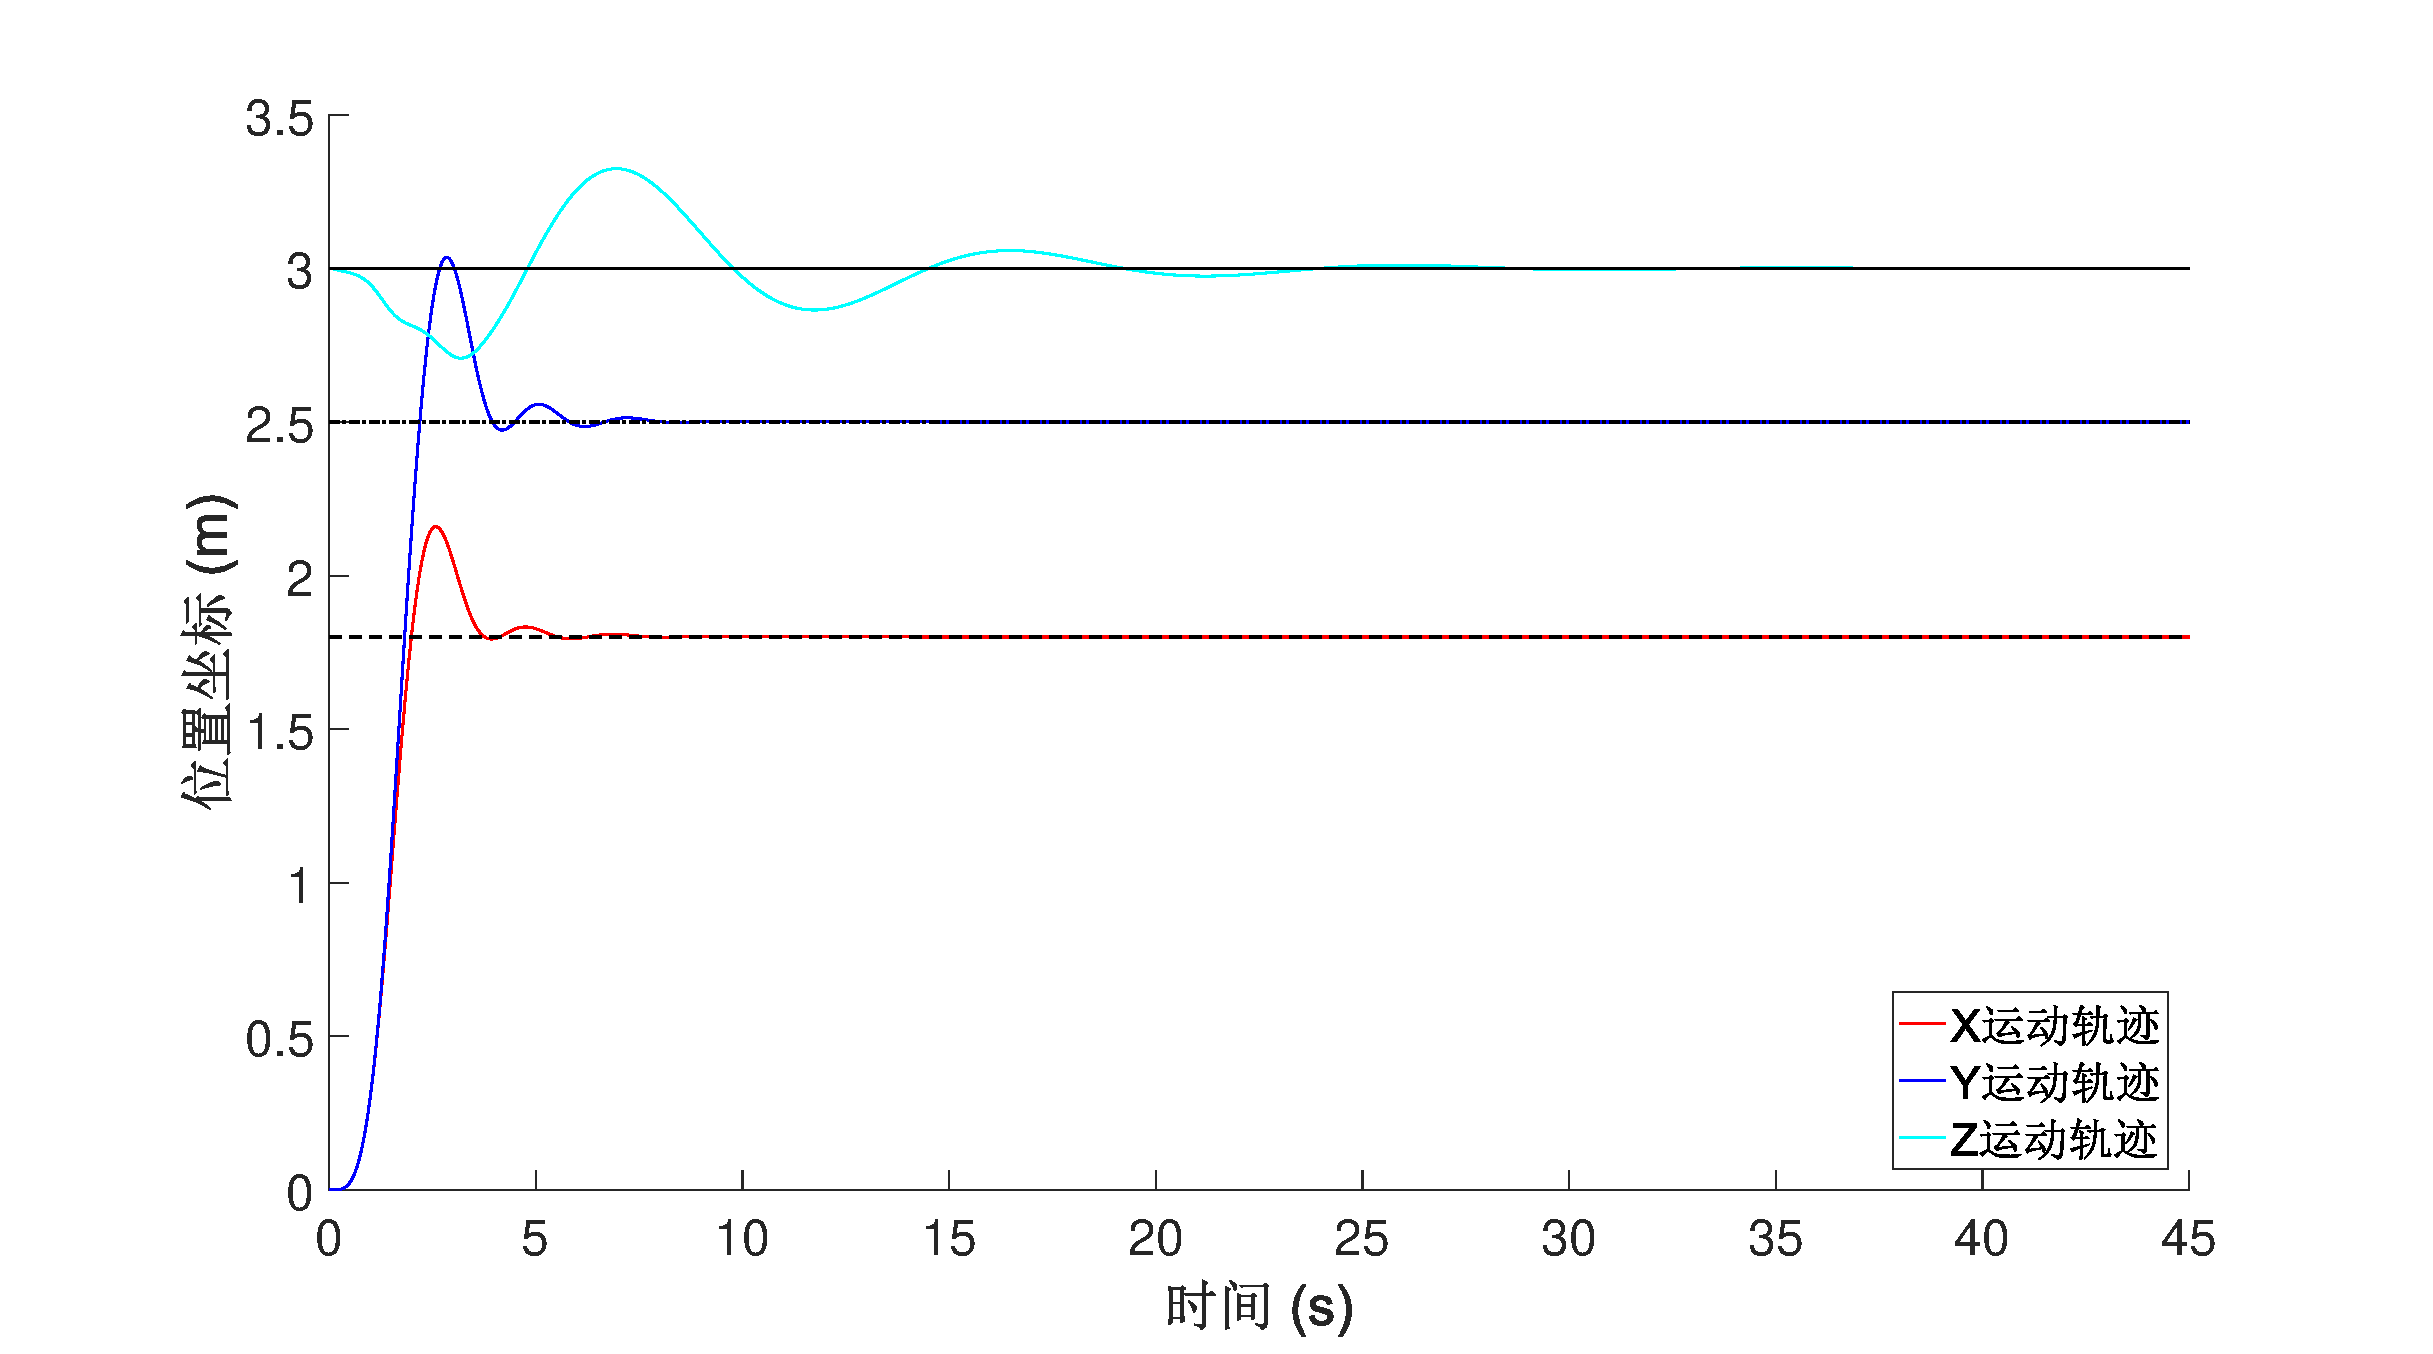
\includegraphics[scale=.18]{figures/Fig2-5_a.eps}
	}
	\subfigure[姿态控制]
    {	
		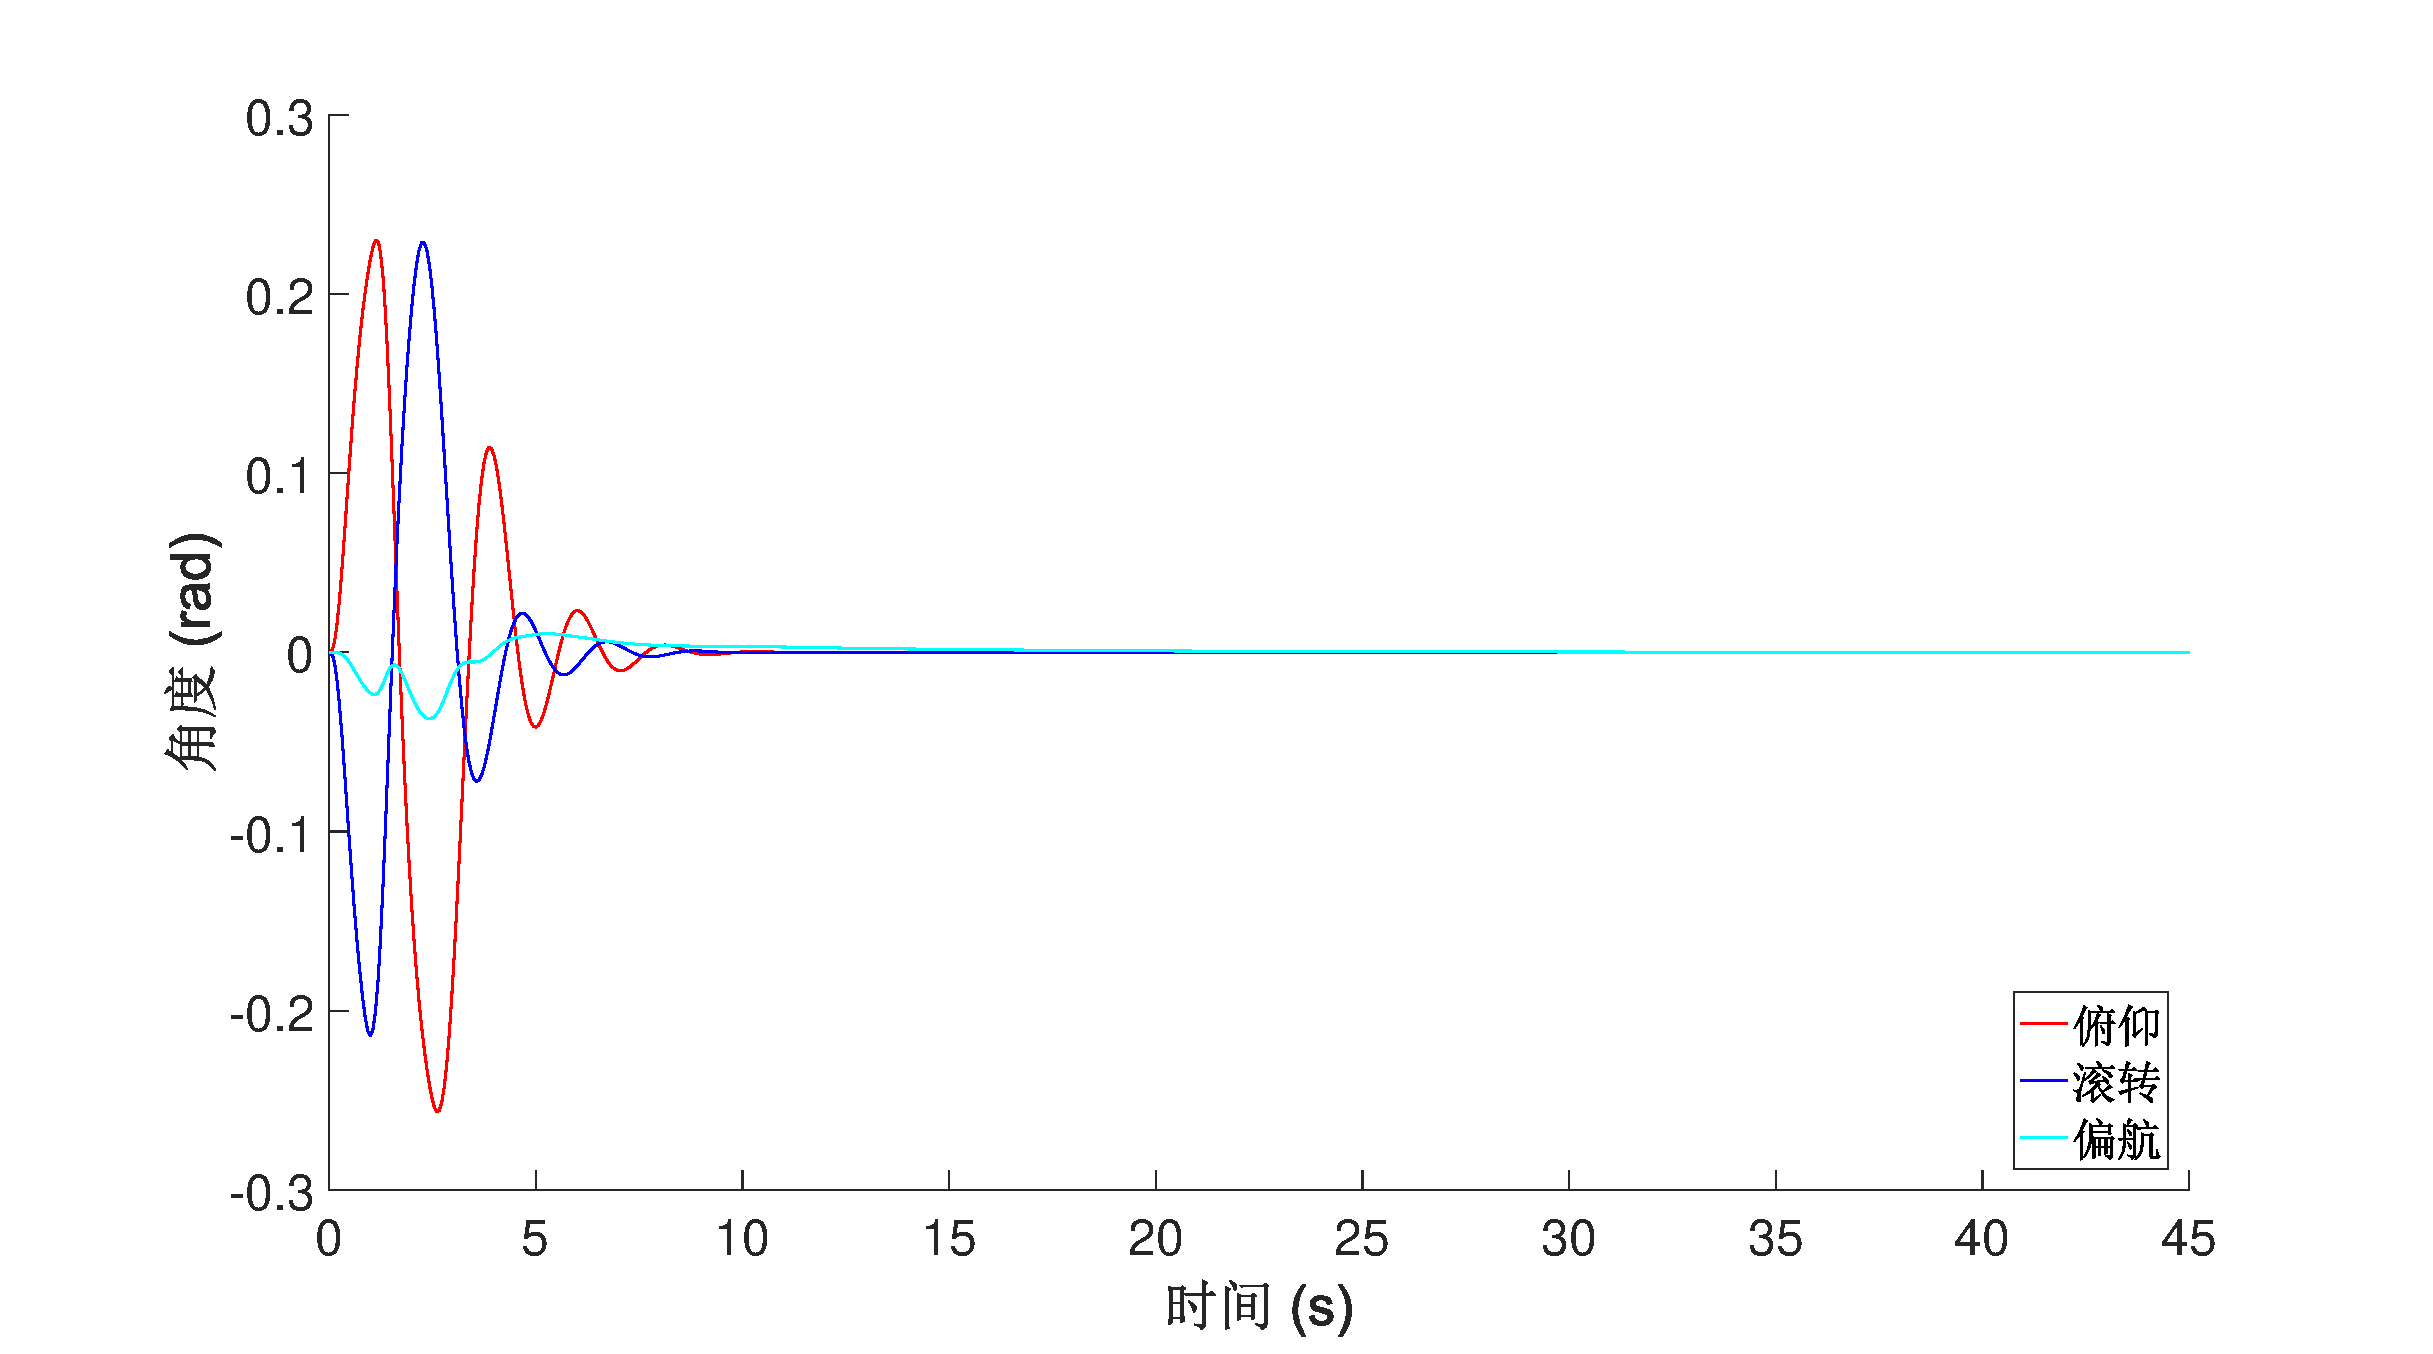
\includegraphics[scale=.18]{figures/Fig2-5_b.eps}
	}
	\subfigure[运动轨迹]
    {	
		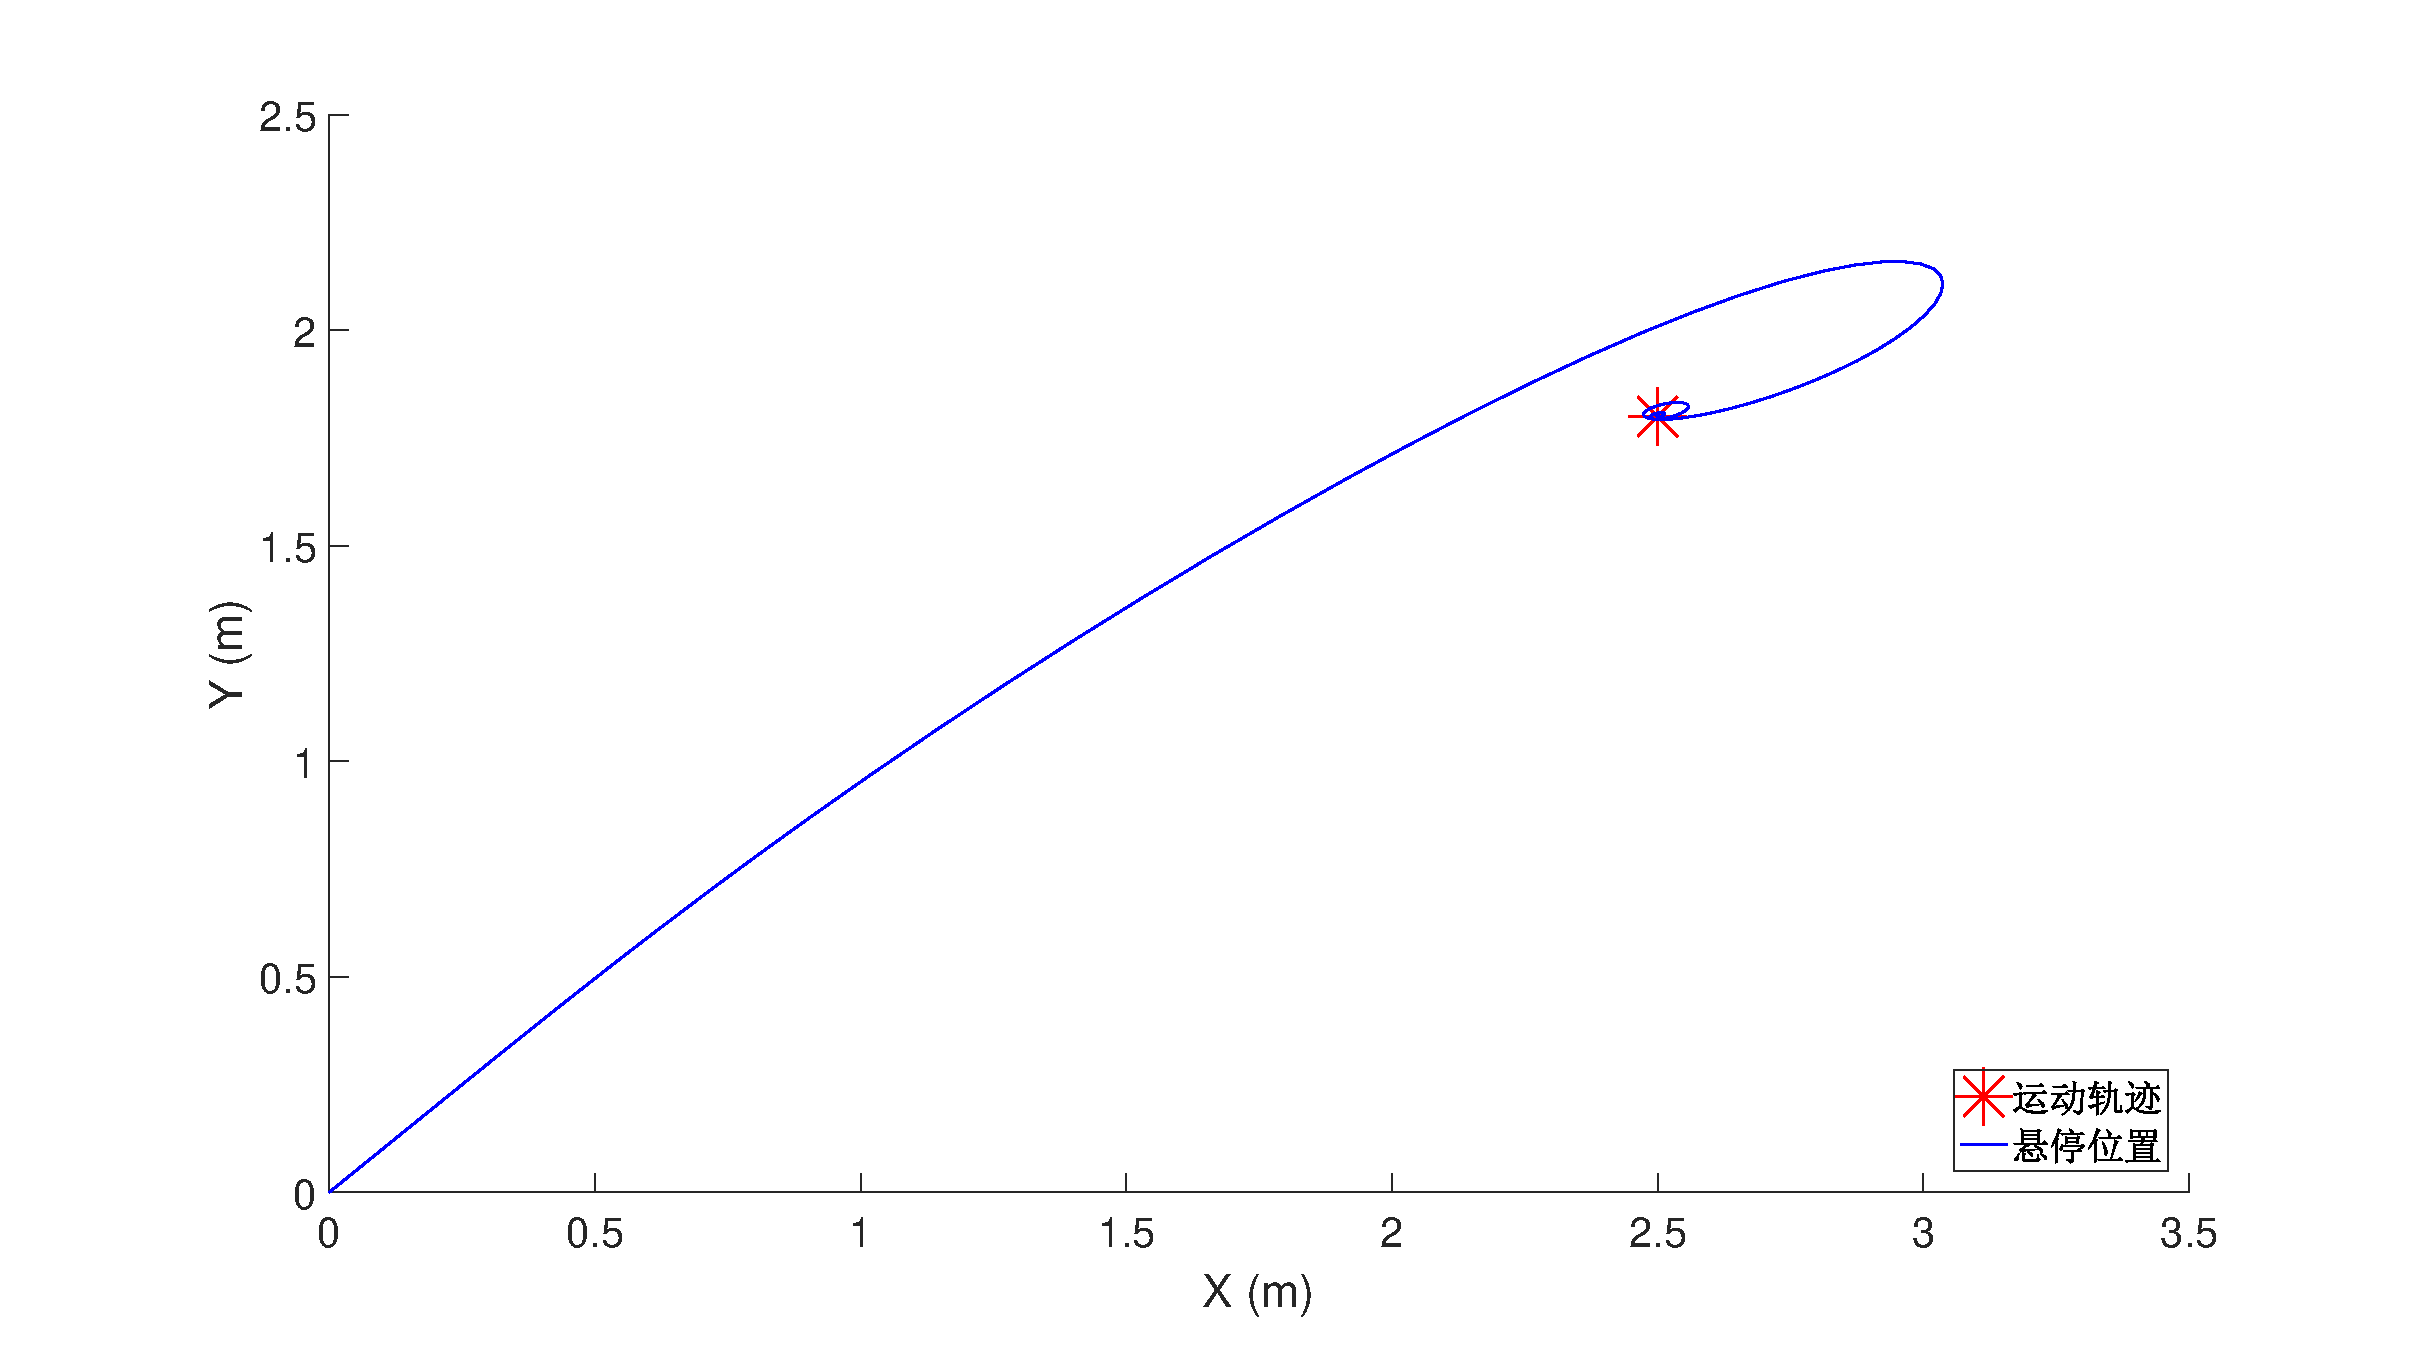
\includegraphics[scale=.2]{figures/Fig2-5_c.eps}
	}
\caption{无人机控制仿真结果}
\label{fig2.5}
\end{figure}


\section{本章小结}
本章主要研究多旋翼无人机的建模和控制系统设计。对无人机的运动学模型和运动学模型的非线性部分进行线性近似和化简,根据简化模型设计串级PID控制器,完成无人机的位置控制和姿态控制。通过MATLAB仿真,验证无人机建模的准确性和控制算法的可行性,了解多旋翼无人机的运动特性,便于之后分析和选择适合无人机的视觉SLAM算法。

